\documentclass[18pt]{beamer}

\usepackage[utf8]{inputenc}
\setbeamertemplate{navigation symbols}{}
\usetheme{Warsaw}
\beamersetuncovermixins{\opaqueness<1>{25}}{\opaqueness<2->{15}}
\usepackage{lmodern}
\usepackage{graphicx,url}
\usepackage{enumerate}
\usepackage{scrextend}
\changefontsizes{7.5pt}

\usepackage[all]{xy}

\begin{document}

  \title{}
  \author{        Denilson Alves Pereira \\ Eduardo Emanuel Braga da Silva}

  

  \institute[UFLA]{
      Departamento de Ciência da Computação\\
      Universidade Federal de Lavras\\

  }

    \date{\today}

  \begin{frame}
	  \titlepage
  \end{frame}




\section{Introdução}  
    
    \subsection{Objetivo}
        \frame{
		    \frametitle{Objetivo}
		    \begin{itemize}
				\item Classificar nomes de Veículos de Publicações.
				\item Ser capaz de reconhecer uma grande variedade de nomes de veículos de publicação.
			    \item Criar um base de dados para treinamento, recolhendo variações dos nomes em bibliotecas digitais.
			    \item Dado uma variação do nome de um veículo, fornece se as informações completas deste veículo.
		    \end{itemize}
		}
	
	\subsection{Motivação}
	    \frame{
			\frametitle{Motivação}
			\begin{itemize}
				\item Um mesmo veículo tratado como sendo diferente.
				\item Dificuldades para fazer pesquisas.
				\item Resultados redundantes nas buscas.
				\item Inconsistência de dados.
		    \end{itemize}
		}

	\subsection{Dificuldades}
		\frame{
				\frametitle{Dificuldades}
				\begin{table}[htb]
				\centering
				\label{tabela2}
				\begin{tabular}{|c|c|}
				\hline
				Nome & Tipo\\
				\hline
				Advances in Software Engineering & J\\
				\hline
				Advances in Engineering Software & J\\
				\hline
				\end{tabular}
				\caption{Dificuldades encontradas.}
				\end{table}
				
				
			}
		\frame{
				\frametitle{Dificuldades}
				\begin{table}[htb]
				\centering
				\label{tabela2}
				\begin{tabular}{|c|c|}
				\hline
				Nome & Tipo\\
				\hline
				Design Automation Conference & C\\
				\hline
				PROC DES AUTOM CONF & C\\
				\hline
				\end{tabular}
				\caption{Dificuldades encontradas.}
				\end{table}
			}

		
	\subsection{Base de Dados}
		\frame{ 
			\frametitle{Coleta dos dados}
			\begin{center}
			\begin{itemize}
			    \item \textit{ACM digital library} 
			    \begin{itemize}
				\item \url{http://dl.acm.org/dl.cfm}
			    \end{itemize}
			    \item \textit{IEEExplore digital library}
			    \begin{itemize}
				\item \url{http://ieeexplore.ieee.org/Xplore/home.jsp}
			    \end{itemize}
			    \item \textit{DBLP computer science library}
			    \begin{itemize}
				\item \url{http://www.informatik.uni-trier.de/~ley/db/}
			    \end{itemize}
			    \item \textit{wikipedia}
			    \begin{itemize}
				\item \url{http://en.wikipedia.org/wiki/List_of_compu}\\
			\url{ter_science_conferences}
			    \end{itemize}
			    \item \textit{Qualis}
			    \begin{itemize}
			    \item \url{http://qualis.capes.gov.br/webqualis/Index.faces}
			    \end{itemize}
			\end{itemize}
			\end{center}	
			
			
		}
		
%		\frame{
%			\frametitle{Modelo XML}
%			
%			\begin{center}
%			\begin{itemize}
%			    \item $<pub-venue>$
%			    \begin{itemize}
%			      \item $<id></id>$
%			      \item $<entity></entity>$
%			      \item $<issn></issn>$
%			      \item $<acronym></acronym>$
%			      \item $<title></title>$
%			      \item $<title-abrev></title-abrev>$
%			      \item $<title-formerly></title-formerly>$
%			      \item $<acronym-formerly></acronym-formerly>$
%			      \item $<merge-of-title></merge-of-title>$
%			      \item $<merge-of-acronym></merge-of-acronym> $
%			      \item $<publisher></publisher>$
%			      \item ...
%			   \end{itemize}
%			   \item $</pub-venue>$
%			\end{itemize}
%			\end{center}
%			
%		}
%		
%				\frame{
%					\frametitle{Modelo XML}
%					
%					\begin{center}
%					\begin{itemize}
%					    \item $<pub-venue>$
%					    \begin{itemize}
%					  	  \item ...
%					      \item $<pub-type></pub-type>$
%					      \item $<language></language>$
%					      \item $<subject></subject>$
%					      \item $<impact-factor-2010></impact-factor-2010>$
%					      \item $<impact-factor-5-years></impact-factor-5-years>$
%					      \item $<qualis-estrato></qualis-estrato>$ 
%					      \item $<site></site>$
%					      \item $<year-first-issue></year-first-issue>$
%					      \item $<year-last-issue></year-last-issue>$
%					   \end{itemize}
%					   \item $</pub-venue>$
%					\end{itemize}
%					\end{center}
%					
%				}
		
		\frame{
					\frametitle{Modelo XML}
					
					\begin{center}
						\begin{itemize}
						\item $<pub-venue>$
						\begin{itemize}
							\item $<id>2</id>$
							\item $<idClass>200</idClass>$
							\item $<acronym>FCRC</acronym>$
							\item $<title>Federated Computing Research Conference</title>$
							\item $<pub-type>C</pub-type>$
						\end{itemize}
						\item $</pub-venue>$
						\end{itemize}
					\end{center}
					
				}
		\frame{
							\frametitle{Modelo XML}
							
							\begin{center}
								\begin{itemize}
								\item $<pub-venue>$
								\begin{itemize}
									\item $<id>27</id>$
									\item $<idClass>2027</idClass>$
									\item $<acronym>DCFS</acronym>$
									\item $<title>International Workshop on Descriptional Complexity of Formal Systems</title>$
									\item $<title>Workshop on Descriptional Complexity of Formal Systems</title>$
									\item $<merge-of-title>Descriptional Complexity of Automata, Grammars and Related Structures</merge-of-title>$
									\item $<merge-of-title>Formal Descriptions and Software Reliability</merge-of-title>$
									\item $<merge-of-acronym>DCAGRS</merge-of-acronym>$
									\item $<merge-of-acronym>FDSR</merge-of-acronym>$
									\item $<pub-type>W</pub-type>$
								\end{itemize}
								\item $</pub-venue>$
								\end{itemize}
							\end{center}
							
						}
				
\newcommand{\tab}{$\mid$\hspace{0.2cm}}
\section{Algoritmo}
		\frame{
			\frametitle{Estrutura do Arquivo Invertido}
		\begin{figure}[!htb]
		\advance\leftskip-50cm
	      \centering			
	      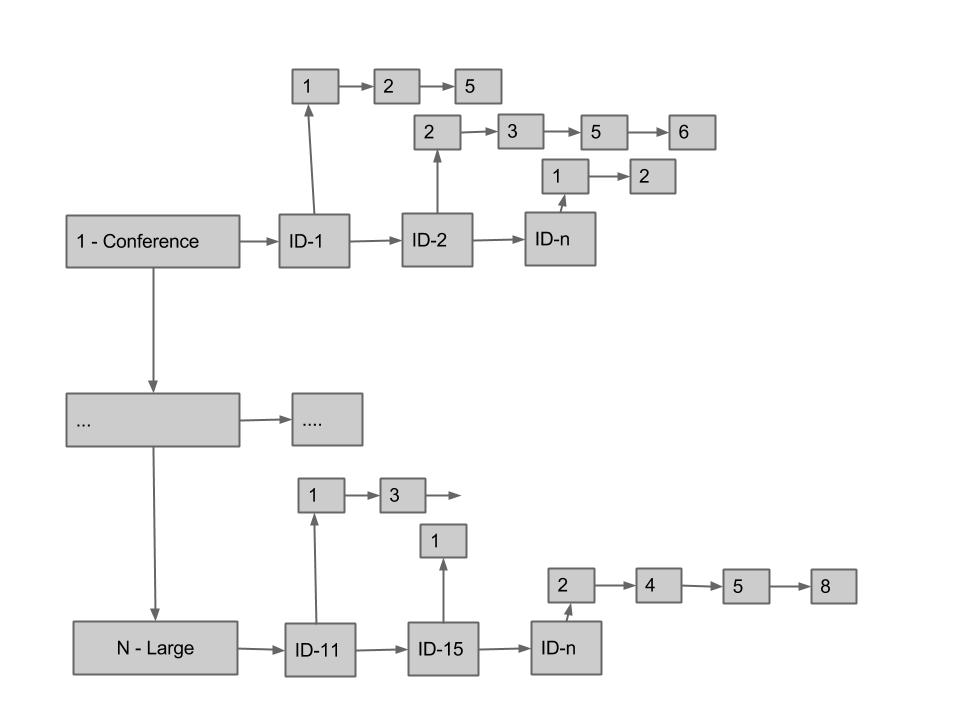
\includegraphics[width=10.0cm,height=7.0cm]{estrutura.jpg}
	      \caption{Estrutura do arquivo invertido.}
	    \end{figure}
			
			
				
			}
			
			\frame{
						\frametitle{Intersecção}
					\begin{figure}[!htb]
					\advance\leftskip-50cm
				      \centering			
				      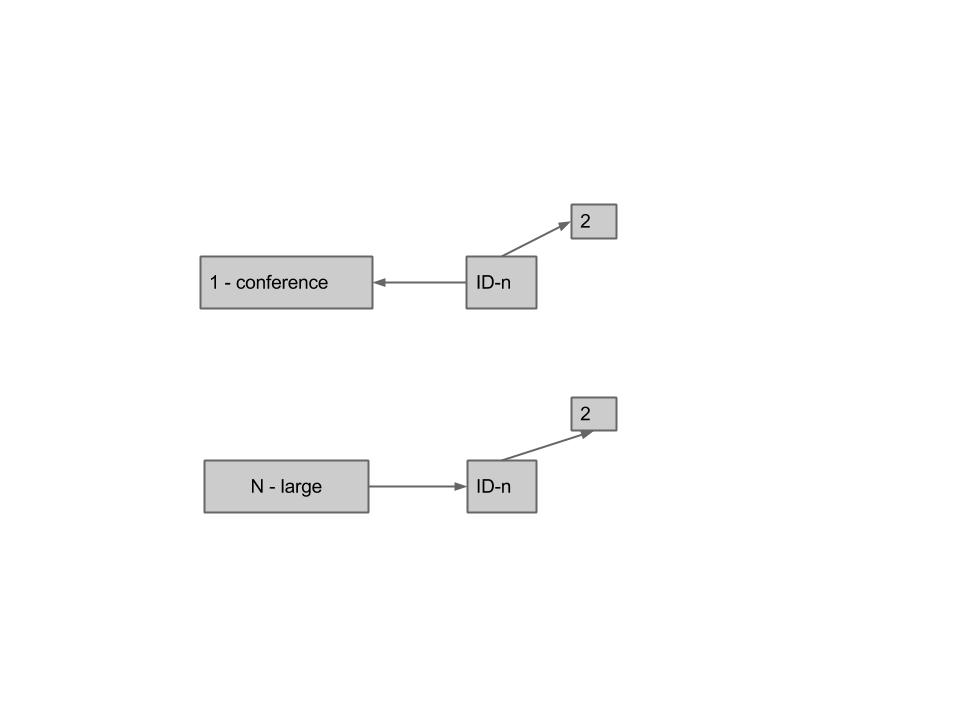
\includegraphics[width=10.0cm,height=7.0cm]{intersect.jpg}
				      \caption{Interseção entre \textit{large e conference}.}
				    \end{figure}
						
						
							
						}
						
						
		\frame{
			\frametitle{Normalização}
				\begin{enumerate}
				\item Substituição dos  delimitadores "\textit{$\backslash$/()\{\}[]\'\ }" por espaço em branco.
				\item Substituição de palavras por outras equivalentes. \textit{syposium - conference}.
				\item Tranformação de letras em maiúsculo para minúsculo.
				\item Remoção de espaços em excesso.
				\item Remoção de qualquer outra pontuação.
				\item Remoção de \textit{stopWords}.
				\end{enumerate}
					
				}
		\frame{
			\frametitle{Algoritmo}

			
			
			
			//Para criar a lista invertida \\
			Para cada veículo nos veículos de treino; faça\\
			\tab Para cada título, sigla e combinação do título e sigla; faça\\
			\tab \tab Normalize e crie os tokens.\\
			\tab \tab Para cada token nos tokens; faça\\
			\tab \tab \tab Insira no  arquivo invertido o token e sua localização.\\
						
			
			//Para criar as regras\\
			Para cada token na lista invertida; faça\\
			\tab Se o token aparecer em apenas um veículo\\
			\tab \tab crie a regra com esse token\\
			\tab Se não\\
			\tab \tab adicione o token em outra lista de itens.\\
			
		}
		\frame{
			\frametitle{Algoritmo}
			\small
			Enquanto a lista de itens não for vazia\\
			\tab Para cada item1 nos itens\\
			\tab \tab Para cada item2 nos itens\\
			\tab \tab \tab se apenas a primeira palavra no item1 e no item2 for diferente; faça\\
			\tab \tab \tab \tab Obtenha a lista de intersecção entre as plavras diferentes\\
			\tab \tab \tab \tab Para as outras palavras do iten1; faça\\
			\tab \tab \tab \tab \tab Enquanto a lista não for vazia; faça \\
			\tab \tab \tab \tab \tab \tab faca a lista igual a interseccao desta lista com a lista da palavra.\\
							
			\tab \tab \tab \tab Se a lista tiver tamanha igual a um\\
			\tab \tab \tab \tab \tab Concatene lexicograficamente a primeira palavra do item2 com o item1 \\
			\tab \tab \tab \tab \tab e verifique se existe uma subregra para este resultado.\\
			\tab \tab \tab \tab \tab Se nao existir crie uma nova regra.\\
								
			\tab \tab \tab \tab Se o tamanho for maior que um\\
			\tab \tab \tab \tab \tab Concatene lexicograficamente o iten1 e o iten2 e adicione em novosItens.\\
								
			\tab Faça itens igual a novos itens	\\
		}						
			
		\frame{
			\frametitle{Algoritmo}		
			//Para fazer o teste\\
			\tab Para cada título a ser classificado; faça\\
			\tab \tab Normalize o título.\\
			\tab \tab Verifique se existe regra para os itensets deste título.\\
			\tab \tab Se existir \\
			\tab \tab \tab Verifique se a similaridade entre o veiculo que aponta a regra e o título é maior que um threshold	\\
			\tab \tab \tab \tab Se for adicione a regra em regras encontradas\\
				
			\tab Se foi encontrada pelo menos uma regra então \\
			\tab \tab Obtenha a com maior similaridade e classifique o título.\\
			\tab Se nenhuma regra foi econtrada\\
			\tab \tab Compare o título com toda a base e classifique pela maior similaridade.\\
		}	
		
\section{Complexidade}
	\frame{
		\frametitle{Complexidade}
		
		
		
		
		}
		
\section{Resultados}
	\frame{
		\frametitle{Resultados}
		
	
	
	}
			

		
		
			
					
				
				
				
				
			
			
				
				
				
			
			
			
				
			
			
			
			
			
			
		
		
		
		
		
	






\end{document}



